\section{Analysis and Results}
\label{sec:description_3}

%\subsection{$2$ Player Game}
%\label{subsec:2playergame}

\subsection{$3$ Player Game}
\label{subsec:3playergame}

\subsubsection{The captain proposes: $(99, 0, 1)$}
\label{subsubsec:3playergame99}

The outcome $CDC$ with a proposal of $(\alpha_{1}, \alpha_{2}, \alpha_{3}) =(99, 0, 1)$ would represent the Nash Equilibrium of the classic Pirate Game (for $3$ players). 

When the players chose at least $2$ operators $Cooperate$ on the initial proposal the game ends right away, the disentangle operator $\mathcal{J}^{\dagger}$ is applied, and the payoff functionals are calculated given the final state. The final state will be calculated as shown in Equation \ref{eq:piratas_final_move2_99anal}. 

The Tables \ref{tab:3playerCCC99}, \ref{tab:3playerCCD99}, \ref{tab:3playerCDC99}, and \ref{tab:3playerDCC99}, in the Apendix \ref{ap:d}
,present the results for the sittuation described above.

In the Table \ref{repro:1} we find a reproduction of Table \ref{tab:3playerCCC99}, where the $3$ players choose to use the cooperate strategy. We can see that the parameter $\gamma$ has no effect on the final result. This happens because no player chooses to change her qubit. 

In Tables \ref{tab:3playerCCD99}, \ref{tab:3playerCDC99}, and \ref{tab:3playerDCC99} we can see a pattern on the probability distributions 
associated with probability of measuring a determined outcome. 

The Table \ref{repro:2} reproduces the results of Table \ref{tab:3playerCDC99}. 
The players select the operators $(CDC)$ in Table \ref{repro:2}, as there two players chose the ``Cooperate'' operator (represented by a $2 \times 2$ identity matrix), the proposal is accepted and the game ends (refer to Figure \ref{fig:pg_architecture3players_architecture}). The states $CDC$ and $DCD$ vary with $\gamma$, such that $P(CDC)= 1 - P(DCD)$. The probability distribution associated with $DCD$(the state where the qubits are flipped ), is approximated by normal distribution as vary $\gamma$. The peak for this distribution happens when the initial system is maximally entangled, for $\gamma=frac{\pi}{2}$.

For $\gamma = 0 + k \pi, k \in \{0,1\}$ we are rendered with the classical situation, this means the proposal suggested by the captain will be enforced exactly as she stated. When $\gamma = \frac{\pi}{2}$ we are before a symmetric outcome where player 1 would die and player 2 would approve her proposal and get the $100$ coins.


\begin{equation}
\label{eq:piratas_final_move2_99anal}
\vert\psi_{fin}\rangle= \mathcal{J}^{\dagger}\vert\psi_{1}\rangle
\end{equation}



 
\begin{table}
\begin{center}
\begin{tabular}{cc}
  a)\putindeepbox[7pt]{\includegraphics[scale=0.46]{3Accepted99/CCC.PNG}}
    & a1)\putindeepbox[7pt]{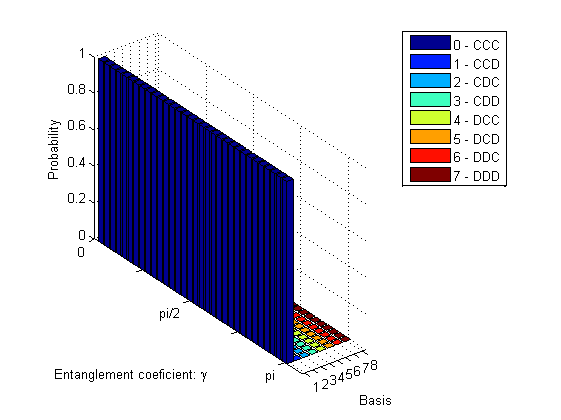
\includegraphics[scale=0.46]{3Accepted99/CCC_1.PNG}} \\
\end{tabular}
\caption{a) Expected utility for $3$ players, where the players will use the $(Cooperate, Cooperate, Cooperate)$ operators. The initial proposal is $(\alpha_{1}, \alpha_{2}, \alpha_{3}) =(99, 0, 1)$. a1) Probability distribution of the final state depending on the entanglement coefficient $\gamma$.  Reproduction from Table \ref{tab:3playerCCC99}}
\label{repro:1}
\end{center}
 \end{table}

\begin{table}
\begin{center}
\begin{tabular}{cc}
  b)\putindeepbox[7pt]{\includegraphics[scale=0.46]{3Accepted99/CDC.PNG}}
    & b1)\putindeepbox[7pt]{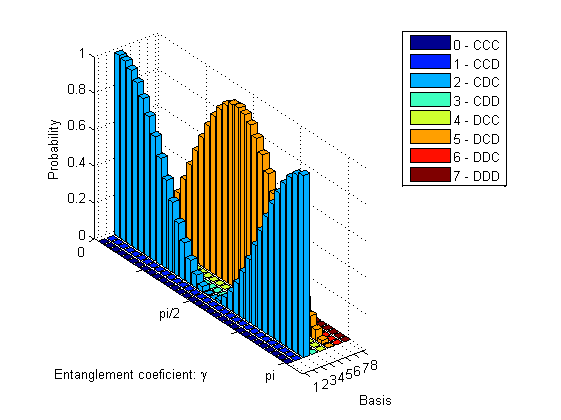
\includegraphics[scale=0.46]{3Accepted99/CDC_1.PNG}} \\
\end{tabular}
\caption{b) Expected utility for $3$ players, where the players will use the $(Cooperate, Defect, Cooperate)$ operators. b1) Probability distribution of the final state depending on the entanglement coefficient $\gamma$.  Reproduction from Table \ref{tab:3playerCDC99}.}
\label{repro:2}
\end{center}
 \end{table}

When the first proposal is rejected (more than $1$ player chooses to $Defect$), the second round ensues. We calculate the final state for these states with Equation \ref{eq:piratas_final_move2_99anal1}. 


\begin{equation}
\label{eq:piratas_final_move2_99anal1}
\vert\psi_{fin}\rangle= \mathcal{J}^{\dagger}\vert\psi_{2}\rangle
\end{equation}

In a classical game the best response for player $1$ is to cooperate. In this quantum version depending of the parameter $\gamma$, the strategy that produces the most favourable outcome changes. However if the first proposal is rejected and player $1$ voted in favour (using the $C$ operator), we get to a final sub-game where the parameter $\gamma$ won't influence the expected utility; these results for this can be consulted on Appendix \ref{ap:d}, Section \ref{ap:d:CDD99}. Table \ref{repro:3} displays a particular outcome of the sub-game generated when the players chose the operators $CDD$ in the first stage ($CD$); it shows the expected utility when player $2$ accepts her proposal, and player $3$ rejects. 

This happens due to the nature of the game, more specifically the way we calculate our expected utility for each player, which is described in Section \ref{subsec:pirates_utility}, Equation \ref{eq:pirates_payoff32}. The sum of the probability for the system being on states $\vert CCD\rangle$ or $\vert CDC\rangle$ is constant ($\frac{1}{2}$), this also happens with the sum of the probability of the system being on state $vert DCD\rangle$ or $\vert DDC\rangle$.

However the parameter $\gamma$ affects the probability of the system being measured in a determined state, as in Table \ref{repro:3}.

 \begin{table}[h]
\begin{center}
\begin{tabular}{cc}
  c)\putindeepbox[7pt]{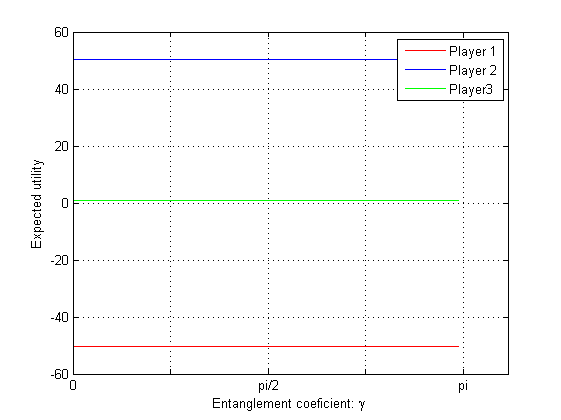
\includegraphics[scale=0.46]{3Rejected99/CDD_CD.PNG}}
    & c1)\putindeepbox[7pt]{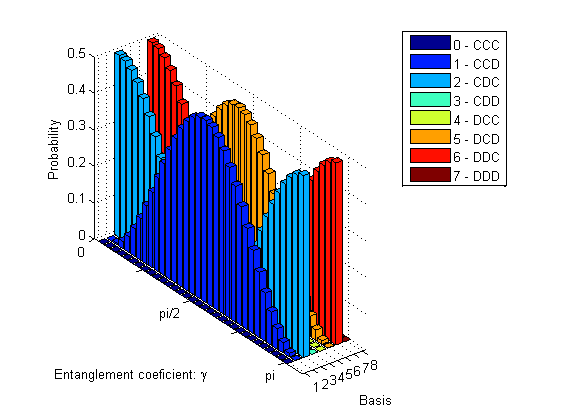
\includegraphics[scale=0.46]{3Rejected99/CDD_CD1.PNG}} \\
\end{tabular}
\caption{Expected utility for $3$ players, where the players will use the $(Cooperate , Defect, Defect)$ operators in the first round of the game; in the second round player 2 and player 3 will play $(CD)$.}
\label{repro:3}
\end{center}
 \end{table}

If in the quantum game the player $1$ decides to defect $D$ and the proposal is rejected we get $4$ different probability distributions that are permuted given the players chosen operators. In Tables \ref{tab:3playerDCD_DC99}, 
\ref{tab:3playerDDC_CD99}, and \ref{tab:3playerDDD_CC99} (in Apendix \ref{ap:d})

In Table \ref{tab:3playerDCD_DC99}, the player $2$ has assumes the strategy $\tau_{2}=(C,D)$, this means that she will play $C$ on the first stage and $D$ on the second stage; In Table \ref{tab:3playerDDC_CD99} her strategy is $\tau_{2}=DC$. As the multiplication by a identity matrix is commutative, in the previous cases, we applied the same operation to player $2$ qubit. This result happens because the players are manipulating their qubits with permutation operators $C$ and $D$; described on Section \ref{subsec:strategic_space}, where we define the strategic space the players have access.

When the parameter $\gamma$ influences the expected utility for the players, we verify the functions that describe the expected utility for player $1$ and $3$ tend have maxima and minima for the same values of $\gamma$. However if player $1$ decides to $Defect$ the two functions will not be synchronized.
The function that describes the expected utility for player $2$ tends to have opposite behaviour. This happens because the captain bribed player $3$ with one gold coin.

\subsubsection{The captain proposes: $(100, 0, 0)$}
\label{subsubsec:3playergame100}

Suppose captain is greedy and proposes to get the 100 coins. In the classical Pirate Game this would pose a conflict with his self-preserving needs. 
A pertinent question would be if this Quantum Model of the Pirate Game would allow the first captain to approve that allocation proposal. The initial proposal will be accepted if there is at least $2$ players play $\mathcal{U}_{i}=C$ in a round. 

The player $1$, the captain, needs two votes to pass her proposal. In order to answer our question we must analyse the expected utilities for all players where the initial proposal is accepted. Moreover we need to analyse an instance where the proposal is refused, when the players select the actions $(C,D,D)$. In the previous analysis we observed that player $2$ has a strong motivation to Defect in the first round, because in the second round she can pass the proposal with her vote alone, this means if the player $1$ wants to pass is proposal she should choose the $C$ operator.

 Our final state will be calculated as shown in Equation \ref{eq:piratas_final_move2_99anal}.

In Table \ref{tab:3playerDCC100} we notice that player $3$ will get a expected payoff of $0.5$ if she chooses to Defect.
\begin{table}[h]
\begin{center}
\begin{tabular}{cc}
  \putindeepbox[7pt]{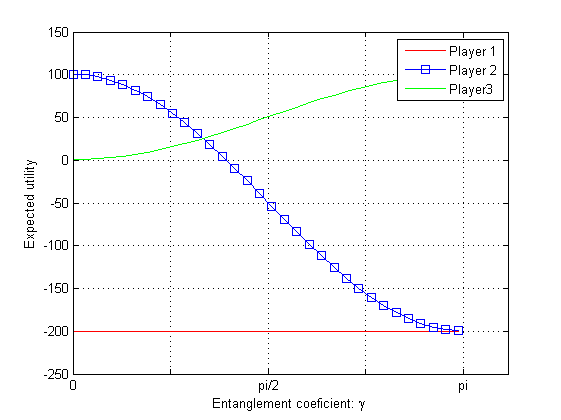
\includegraphics[scale=0.72]{3Accepted100/CDD_CC.PNG}}
\end{tabular}
\caption{Expected utility for $3$ players, where the players will use the $(Cooperate, Defect, Defect)$ operators in the first stage. In the second stage we represented the sub-game equilibrium of the game.  }
\label{tab:3playerDCC100}
\end{center}
 \end{table}


In Tables \ref{tab:3playerCDC100} and \ref{tab:3playerCCD100}, the expected utility function for player $3$ starts of as $0$ for $\gamma=0$ (which corresponds to the classical problem). The function presents a maximum when the system is maximally entangled; this maximum is $0.5$. If the proposal is accepted when the entanglement coefficient is $\gamma=\frac{\pi}{2}$ player $1$ will get a negative expected payoff (which means he will die under that condition).

\begin{table}[h]
\begin{center}
\begin{tabular}{c}
  \putindeepbox[7pt]{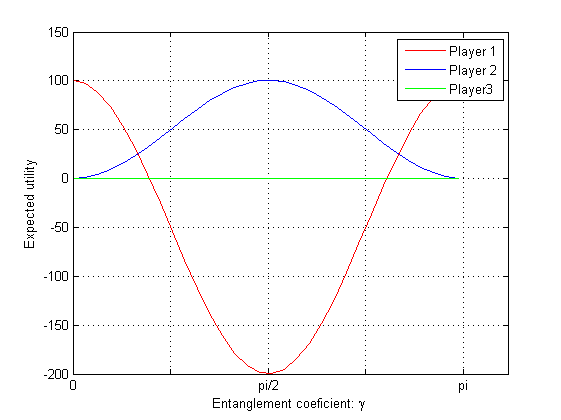
\includegraphics[scale=0.72]{3Accepted100/CCD.PNG}}
\end{tabular}
\caption{Expected utility for $3$ players, where the players will use the $(Cooperate, Cooperate, Defect)$ operators. }
\label{tab:3playerCCD100}
\end{center}
 \end{table}

\begin{table}[h]
\begin{center}
\begin{tabular}{c}
  \putindeepbox[7pt]{\includegraphics[scale=0.72]{3Accepted100/CDC.PNG}}
   
\end{tabular}
\caption{Expected utility for $3$ players, where the players will use the $(Cooperate, Defect, Cooperate)$ operators.}
\label{tab:3playerCDC100}
\end{center}
 \end{table}

The Table \ref{tab:3playerCCC100} presents an outcome where all the players vote in favour of the proposal. The players $2$ and $3$ have and expected utility of $0$, regardless the role of entanglement in the system.



\begin{table}[h]
\begin{center}
\begin{tabular}{c}
  \putindeepbox[7pt]{\includegraphics[scale=0.72]{3Accepted100/CCC.PNG}}
\end{tabular}
\caption{Expected utility for $3$ players, where the players will use the $(Cooperate, Cooperate, Cooperate)$ operators. The initial proposal is $(\alpha_{1}, \alpha_{2}, \alpha_{3}) =(100, 0, 0)$. }
\label{tab:3playerCCC100}
\end{center}
 \end{table}

From this simulation we can conclude that if the captain wants to pass her proposal for $\gamma=\frac{\pi}{2}$ there are $3$ equilibria when the player select the operators $(CDC)$, $(C,C,D)$, and $((C,D,D),(C,C))$. $(CDC)$, $(C,C,D)$ correspond to an accepted proposal. However player $1$ will get a negative payoff in any of this equilibria. 

We can interpret this in the context of the problem with the captain getting the coins as she proposed, but being immediately betrayed and killed by her fellow pirates who conspired in order for player $2$ to get all the coins, and player $3$ to become second in command.

Otherwise there is one Nash Equilibrium when the players select $((C,D,D),(C,C))$. Even in a quantum version, the captain needs to bribe player $3$ in order to approve her proposal and get a maximum of $99$ gold coins.







